% ----------------------------------------------------
\begin{frame}
  \titlepage
\end{frame}
% ----------------------------------------------------
\note{Introducción a la sesión. Conectar con la sesión anterior sobre normas y derecho internacional. Hoy pasamos de la seguridad a la economía política internacional. El comercio es el tema más antiguo de la economía política: ¿por qué intercambian los países? ¿Quién gana y quién pierde? ¿Por qué los gobiernos ponen trabas a algo que, según los economistas, genera ganancias netas? Cuatro bloques: el rompecabezas básico, ventaja comparativa, ganadores y perdedores, y la política del proteccionismo y la cooperación.}

% ----------------------------------------------------
\begin{frame}
\frametitle{Hoy}
\centering
\vspace{1.5em}
\begin{itemize}
  \setlength{\itemsep}{10pt}
  \item El rompecabezas del comercio: ganancias netas, pero restricciones
  \item Ventaja comparativa y patrones de comercio internacional
  \item Ganadores y perdedores del libre comercio
  \item Proteccionismo: tipos y lógica política
  \item Cooperación internacional: GATT y OMC
  \item El trilema de la globalización (Rodrik)
\end{itemize}
\end{frame}
% ----------------------------------------------------
\note{}

% ====================================================
\section{El rompecabezas}
% ====================================================

% ----------------------------------------------------
\begin{transitionframe}
El rompecabezas del comercio
\end{transitionframe}
% ----------------------------------------------------
\note{}

% ----------------------------------------------------
\begin{frame}[plain]
  \begin{tikzpicture}[remember picture, overlay]
    \node[at = (current page.center), yshift = 0cm] (cover) {%
      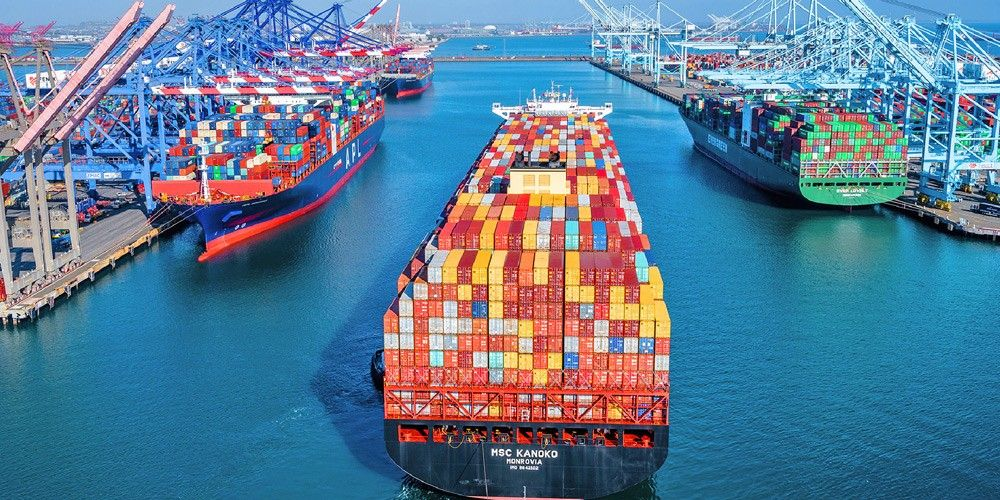
\includegraphics[keepaspectratio, height=\paperheight]{../img/container_ship.jpg}};
  \end{tikzpicture}
\end{frame}
% ----------------------------------------------------
% IMAGE NEEDED: container_ship.jpg -- fotografía aérea de un gran buque portacontenedores en alta mar o en un puerto; preferiblemente con grúas de carga al fondo para subrayar la escala del comercio global
\note{Imagen de apertura. El comercio internacional es la espina dorsal de la economía global. Los barcos portacontenedores mueven el 90\% del volumen del comercio mundial. Sin este sistema, los teléfonos, la ropa, los coches y gran parte de los alimentos que consumimos no existirían a los precios que conocemos. La pregunta fundamental de hoy: si el comercio es tan beneficioso, ¿por qué todos los países lo restringen?}

% ----------------------------------------------------
\begin{frame}
\frametitle{El rompecabezas}
\centering

\begin{itemize}
  \item Los economistas coinciden: el \textbf{libre comercio genera ganancias netas} para la economía
  \item<2-> Sin embargo, \alert{todos los países restringen el comercio} --- aranceles, cuotas, subsidios
  \item<3-> El caso del acero en EE.UU.:
  \begin{itemize}
    \item $\sim$80.000 trabajadores protegidos por aranceles al acero
    \item Coste para los consumidores: miles de millones de dólares al año
    \item Coste por puesto de trabajo ``salvado'': varios cientos de miles de dólares
  \end{itemize}
  \item<4-> \textbf{Pregunta central:} ¿por qué gobiernan los perdedores sobre los ganadores?
\end{itemize}

\end{frame}
% ----------------------------------------------------
\note{El caso del acero es el ejemplo de libro de FLS. En los años 2000, los aranceles de Bush al acero (2002) protegían a los trabajadores siderúrgicos, pero el coste para las industrias que usan acero (automóviles, construcción, electrodomésticos) era enorme. La OMC falló contra los aranceles y Bush los retiró en 2003. Trump volvió a imponerlos en 2018. La paradoja básica: si el libre comercio genera más riqueza total, ¿por qué los gobiernos no simplemente compensan a los perdedores y se quedan con las ganancias netas? La respuesta tiene que ver con política, no con economía.}

% ----------------------------------------------------
\begin{frame}
\frametitle{Comercio: ganancias y redistribución}
\centering
\vspace{0.5em}

\begin{tikzpicture}[>=stealth, thick]
  % Total pie concept
  \node[draw, fill=accent!20, rounded corners, minimum width=3.5cm, minimum height=1.1cm, align=center] (A) at (0,0)
    {\textbf{Libre comercio}\\\small pastel más grande};
  \node[draw, fill=accent2!20, rounded corners, minimum width=3.5cm, minimum height=1.1cm, align=center] (B) at (7,0)
    {\textbf{Proteccionismo}\\\small pastel más pequeño};

  \draw[->, thick, dashed] (A) -- node[above, font=\small]{¿por qué no?} (B);

  \node[align=center, font=\small, text=accent] at (0,-1.6)
    {Ganadores: muchos\\pero ganan poco cada uno};
  \node[align=center, font=\small, text=accent2] at (7,-1.6)
    {Ganadores: pocos\\pero ganan mucho cada uno};
\end{tikzpicture}

\vspace{10pt}
\onslide<2->{\small El comercio crea \textbf{ganadores y perdedores} --- y los perdedores están \textbf{mejor organizados}}

\end{frame}
% ----------------------------------------------------
\note{El punto central del capítulo: el comercio genera ganancias netas (el pastel global crece), pero no distribuye esas ganancias de forma uniforme. Hay sectores e individuos que pierden, y esos perdedores tienen incentivos muy fuertes para organizarse y presionar a los gobiernos. Los consumidores, que se benefician de precios más bajos, son muchos pero difusos: cada uno gana poco, por lo que no merece la pena dedicar tiempo y dinero a presionar. Los productores de un sector específico, en cambio, tienen mucho que perder o ganar y están concentrados geográficamente, lo que facilita la organización.}

% ----------------------------------------------------
\begin{frame}
\centering
\vspace{2em}
{\large Si el libre comercio genera más riqueza total,\\[10pt]
¿por qué los gobiernos no compensan a los perdedores\\[6pt]
y se quedan con las ganancias netas?}
\end{frame}
% ----------------------------------------------------
\note{Pausa socrática antes de entrar en la teoría. Dejar que los estudiantes reflexionen 30 segundos y dar la palabra a 2-3. La respuesta viene en la segunda mitad del tema (acción colectiva, política doméstica), pero conviene que los estudiantes lleguen a la teoría con esta pregunta en mente.}

% ====================================================
\section{Ventaja comparativa}
% ====================================================

% ----------------------------------------------------
\begin{transitionframe}
Ventaja comparativa y patrones de comercio
\end{transitionframe}
% ----------------------------------------------------
\note{}

% ----------------------------------------------------
\begin{frame}
\frametitle{¿Por qué comercian los países?}
\centering

\begin{itemize}
  \item \textbf{Ricardo (1817):} \alert{ventaja comparativa}
  \begin{itemize}
    \item Un país debe especializarse en lo que produce con menor coste relativo
    \item Aunque sea peor en todo, gana especializándose y comerciando
  \end{itemize}
  \item<2-> Ejemplo clásico: Portugal produce tela y vino más eficientemente que Inglaterra
  \begin{itemize}
    \item Pero Portugal tiene ventaja comparativa en vino
    \item Inglaterra tiene ventaja comparativa en tela
    \item Ambos ganan especializándose
  \end{itemize}
  \item<3-> Implicación: el comercio es un juego de \textbf{suma positiva}
\end{itemize}

\end{frame}
% ----------------------------------------------------
\note{La ventaja comparativa es una de las ideas más contraintuitivas y sólidas de la economía. David Ricardo la formuló en 1817 para defender el libre comercio de granos en Inglaterra. El principio: lo que importa no es la ventaja absoluta (ser el mejor en algo), sino la ventaja relativa (el coste de oportunidad). Si Portugal es dos veces más eficiente en vino y solo un 20\% más eficiente en tela, le sale mejor dedicarse al vino y comprar tela a los ingleses. El resultado: producción total mundial mayor. El problema es que la ventaja comparativa dice que el comercio es beneficioso en términos netos, pero no dice nada de cómo se distribuyen esas ganancias. Esa es la parte políticamente explosiva.}

% ----------------------------------------------------
\begin{frame}
\frametitle{Heckscher-Ohlin: dotación de factores}
\centering

\begin{itemize}
  \item \textbf{H-O (1919/1933):} los países exportan bienes que usan intensivamente sus \textbf{factores abundantes}
  \vspace{8pt}
  \item Tres factores de producción: \textbf{tierra}, \textbf{trabajo} y \textbf{capital}
  \vspace{8pt}
  \item<2-> Ejemplos:
  \begin{itemize}
    \item Países con mucha tierra y poco trabajo $\rightarrow$ exportan cereales (EE.UU., Argentina)
    \item Países con mano de obra barata $\rightarrow$ exportan manufacturas (China, Bangladesh)
    \item Países con mucho capital $\rightarrow$ exportan maquinaria y tecnología (Alemania, Japón)
  \end{itemize}
  \item<3-> Predice qué produce y exporta cada país según su \textbf{dotación de recursos}
\end{itemize}

\end{frame}
% ----------------------------------------------------
\note{El modelo Heckscher-Ohlin es más operativo que Ricardo porque predice qué bienes concretos exportará cada país. Desarrollado por el sueco Eli Heckscher (1919) y su alumno Bertil Ohlin (1933). La idea básica: si un país tiene mucho capital y poco trabajo, producir bienes intensivos en capital (maquinaria, tecnología) le resulta relativamente barato, y esos son los bienes que exportará. El modelo tiene implicaciones políticas directas: si China tiene abundancia de trabajo barato y EE.UU. de capital cualificado, el libre comercio beneficia al trabajo chino y al capital americano. Pero perjudica al trabajo americano (que compite con el chino) y al capital chino. Esto conecta directamente con el debate sobre el impacto del comercio en los salarios de los trabajadores no cualificados en los países ricos.}

% ----------------------------------------------------
\begin{frame}
\frametitle{Patrones del comercio mundial}
\centering
\vspace{0.3em}

\begin{columns}[T]
  \begin{column}{0.47\textwidth}
    \centering
    \textbf{\textcolor{accent}{H-O: comercio inter-industrial}}
    \begin{itemize}
      \item Entre países con dotaciones diferentes
      \item Ej: tela (Bangladesh) $\leftrightarrow$ maquinaria (Alemania)
      \item Explica Norte--Sur
    \end{itemize}
  \end{column}
  \begin{column}{0.47\textwidth}
    \centering
    \textbf{\textcolor{accent2}{Comercio intra-industrial}}
    \begin{itemize}
      \item Entre países similares
      \item Ej: coches alemanes $\leftrightarrow$ coches japoneses
      \item Explica Norte--Norte
      \item Multinacionales, marcas, economías de escala
    \end{itemize}
  \end{column}
\end{columns}

\vspace{10pt}
\onslide<2->{\small Gran parte del comercio moderno es \textbf{intra-industrial}: no predecible por H-O}

\end{frame}
% ----------------------------------------------------
\note{El modelo H-O predice bien el comercio Norte-Sur (bienes diferentes entre países con dotaciones muy distintas), pero falla en explicar por qué Alemania exporta coches a EE.UU. y EE.UU. exporta coches a Alemania. Ese comercio intra-industrial es hoy el más voluminoso entre países desarrollados. Las explicaciones: (1) economías de escala: tiene sentido que una planta fabrique un solo modelo para todo el mundo; (2) diferenciación de productos: los consumidores quieren variedad y marcas específicas (BMW vs. Ford); (3) cadenas de valor globales: partes de un mismo coche se fabrican en distintos países. También: geografía y costes de transporte. Los países que comercian más tienden a ser vecinos (gravedad del comercio).}

% ====================================================
\section{Ganadores y perdedores}
% ====================================================

% ----------------------------------------------------
\begin{transitionframe}
Ganadores y perdedores del libre comercio
\end{transitionframe}
% ----------------------------------------------------
\note{}

% ----------------------------------------------------
\begin{frame}
\frametitle{El libre comercio redistribuye}
\centering

\begin{itemize}
  \item El libre comercio genera \textbf{ganancias netas}, pero también \textbf{redistribuye}
  \item<2-> Hay ganadores claros:
  \begin{itemize}
    \item Consumidores (precios más bajos)
    \item Sectores exportadores y sus trabajadores
    \item Propietarios del factor abundante
  \end{itemize}
  \item<3-> Y perdedores claros:
  \begin{itemize}
    \item Sectores que compiten con importaciones
    \item Trabajadores de esos sectores
    \item Propietarios del factor escaso
  \end{itemize}
  \item<4-> La política del comercio es la política de \alert{quién paga la redistribución}
\end{itemize}

\end{frame}
% ----------------------------------------------------
\note{Este es el punto de partida de la economía política del comercio. El libre comercio no es neutral: crea ganadores y perdedores. La teoría del bienestar dice que se podría compensar a los perdedores con parte de las ganancias de los ganadores y aún así todo el mundo estaría mejor. Pero esa compensación raramente ocurre en la práctica. La política del comercio es, en última instancia, una batalla distributiva sobre quién se queda con qué parte del pastel.}

% ----------------------------------------------------
\begin{frame}
\frametitle{Stolper-Samuelson: el factor escaso pierde}
\centering

\begin{itemize}
  \item \textbf{Stolper-Samuelson (1941):} el libre comercio \alert{perjudica} al factor escaso de un país
  \vspace{8pt}
  \item Lógica:
  \begin{itemize}
    \item País rico en capital, escaso en trabajo $\rightarrow$ libre comercio $\rightarrow$ salarios bajan, rentas del capital suben
    \item País rico en trabajo, escaso en capital $\rightarrow$ libre comercio $\rightarrow$ salarios suben, rentas del capital bajan
  \end{itemize}
  \vspace{8pt}
  \item<2-> Predicción política:
  \begin{itemize}
    \item Trabajadores en países ricos $\rightarrow$ \textbf{proteccionistas}
    \item Capital en países ricos $\rightarrow$ \textbf{librecambistas}
    \item Trabajadores en países pobres $\rightarrow$ \textbf{librecambistas}
  \end{itemize}
\end{itemize}

\end{frame}
% ----------------------------------------------------
\note{El teorema de Stolper-Samuelson (1941) es la aplicación política más directa del modelo H-O. Dice que el libre comercio beneficia al factor abundante y perjudica al factor escaso. En un país rico como EE.UU., el capital es abundante y el trabajo no cualificado es relativamente escaso (comparado con China o Bangladesh). Por tanto, el libre comercio entre EE.UU. y China debería beneficiar al capital americano (que compite bien) y perjudicar a los trabajadores no cualificados americanos (que compiten con chinos que cobran mucho menos). Esta predicción explica por qué los sindicatos en los países ricos suelen ser proteccionistas, mientras que las grandes empresas tienden a apoyar el libre comercio. También explica el voto pro-Trump en el cinturón del óxido: exactamente los trabajadores de manufacturas que compiten con importaciones chinas.}

% ----------------------------------------------------
\begin{frame}
\frametitle{Ricardo-Viner: los sectores importan}
\centering

\begin{itemize}
  \item \textbf{A diferencia de Stolper-Samuelson:} los factores no se mueven libremente entre sectores (más realista a corto plazo)
  \item \textbf{Modelo de factores específicos (Ricardo-Viner):}
  \begin{itemize}
    \item Los factores no se mueven fácilmente entre sectores
    \item Un trabajador del acero no es fácilmente un programador
  \end{itemize}
  \item<2-> La identidad \textbf{sectorial} importa más que la identidad de \textbf{clase}
  \begin{itemize}
    \item Capitalistas y trabajadores del acero: ambos \textbf{proteccionistas}
    \item Capitalistas y trabajadores de Boeing: ambos \textbf{librecambistas}
  \end{itemize}
  \item<3-> Evidencia: las coaliciones políticas por el comercio cruzan líneas de clase
  \begin{itemize}
    \item Ej: textil americano -- trabajadores y empresarios juntos pidiendo protección
  \end{itemize}
\end{itemize}

\end{frame}
% ----------------------------------------------------
\note{El modelo de factores específicos (también llamado Ricardo-Viner) parte de una premisa realista: el capital y el trabajo no se mueven libremente entre sectores en el corto plazo. Una planta siderúrgica no puede reconvertirse en fábrica de software. Por eso, el interés político no sigue necesariamente las líneas de clase (capital vs. trabajo), sino las líneas sectoriales. Los trabajadores del acero y los propietarios de acerías comparten interés en proteger a su industria. Los trabajadores de Boeing y sus accionistas comparten interés en el libre comercio, que les abre mercados. Esto explica por qué el debate político sobre el comercio en EE.UU. no es simplemente capital vs. trabajo, sino sector exportador vs. sector importador-competidor. Es la base de la teoría de grupos de interés en la política comercial.}

% ----------------------------------------------------
\begin{frame}
\frametitle{Productores vs. consumidores}
\centering

\vspace{0.5em}
{\footnotesize
\begin{tabular}{l p{3.2cm} p{3.2cm}}
 & \textbf{\textcolor{accent}{Libre comercio}} & \textbf{\textcolor{accent2}{Proteccionismo}} \\[6pt]
\hline
\textbf{Consumidores} & Precios más bajos, más variedad & Precios más altos \\[5pt]
\textbf{Productores exp.} & Acceso a mercados exteriores & Costes más altos (insumos) \\[5pt]
\textbf{Productores imp.} & Competencia, posible cierre & Protección, precios altos \\[5pt]
\textbf{Trabajadores exp.} & Más empleo, mejores salarios & Menos demanda exterior \\[5pt]
\textbf{Trabajadores imp.} & Pérdida de empleo & Empleo protegido \\[5pt]
\end{tabular}
}

\vspace{8pt}
\onslide<2->{\small Los productores domésticos tienen \textbf{ganancias concentradas}; los consumidores tienen \textbf{pérdidas difusas}}

\end{frame}
% ----------------------------------------------------
\note{Esta tabla resume quién gana y quién pierde con el libre comercio y el proteccionismo. El punto clave para la política: los productores que compiten con importaciones tienen ganancias muy concentradas si consiguen protección (toda la diferencia de precios va a ellos), mientras que los consumidores sufren pérdidas muy dispersas (cada familia paga unos pocos euros más por sus coches o su ropa). Esta asimetría explica el patrón político básico: los productores organizan grupos de presión eficaces, los consumidores no. El resultado: los gobiernos tienden a conceder protección aunque el coste social sea mucho mayor que el beneficio para el sector protegido.}

% ====================================================
\section{Proteccionismo}
% ====================================================

% ----------------------------------------------------
\begin{transitionframe}
Proteccionismo: tipos y lógica política
\end{transitionframe}
% ----------------------------------------------------
\note{}

% ----------------------------------------------------
\begin{frame}
\frametitle{Instrumentos de protección comercial}
\centering
\vspace{0.3em}

{\footnotesize
\begin{tabular}{>{\bfseries}p{2.5cm} p{4cm} p{2.5cm}}
Instrumento & Mecanismo & Ejemplo \\
\hline
Arancel & Impuesto sobre la importación & Acero EE.UU.\ (25\%) \\[4pt]
Cuota & Límite cuantitativo a las importaciones & Azúcar en la UE \\[4pt]
Subsidio a la exp. & Ayuda pública a exportadores & PAC (UE) \\[4pt]
Barrera no arancelaria & Normas técnicas, sanitarias & Requis.\ fitosanitarios \\[4pt]
Restricción voluntaria & El exportador limita exportaciones & Acuerdo Japón--EE.UU.\ (1981) \\[4pt]
\end{tabular}
}

\vspace{8pt}
\onslide<2->{\small Las \textbf{barreras no arancelarias} son hoy las más importantes y más difíciles de negociar}

\end{frame}
% ----------------------------------------------------
\note{Los cinco instrumentos principales de protección. El arancel es el más transparente y el más fácil de negociar (se puede cuantificar exactamente). Por eso el GATT/OMC ha tenido éxito en reducirlos: de un promedio del 40\% en 1945 al 5\% en los países desarrollados hoy. Las cuotas son más distorsionadoras porque no permiten que el precio ajuste la demanda. Las barreras no arancelarias (BNA) son el campo de batalla actual: normas de seguridad, requisitos de etiquetado, procesos de certificación, que pueden usarse como protección encubierta. Las restricciones voluntarias a la exportación (VER en inglés) son un caso curioso: el exportador acepta limitar sus ventas a cambio de no recibir aranceles; en la práctica, el exportador captura la renta que con un arancel iría al gobierno importador.}

% ----------------------------------------------------
\begin{frame}
\frametitle{¿Por qué existe el proteccionismo?}
\centering

\begin{itemize}
  \item \textbf{Lobbying e intereses concentrados:}
  \begin{itemize}
    \item Los productores se organizan; los consumidores, no
    \item Colson: ``las minorías organizadas derrotan a las mayorías silenciosas''
  \end{itemize}
  \vspace{-2pt}
  \item<2-> \textbf{Argumentos ``válidos'':}
  \begin{itemize}
    \item \textit{Industria naciente:} proteger hasta que sea competitiva
    \item \textit{Seguridad nacional:} no depender del exterior para bienes estratégicos
    \item \textit{Comercio estratégico:} capturar oligopolios globales
  \end{itemize}
  \vspace{-2pt}
  \item<3-> \textbf{Falacias neo-mercantilistas:}
  \begin{itemize}
    \item ``Las exportaciones son buenas, las importaciones son malas''
    \item ``El déficit comercial es una derrota''
  \end{itemize}
\end{itemize}

\end{frame}
% ----------------------------------------------------
\note{El proteccionismo persiste por varias razones. La más importante políticamente: el problema de acción colectiva. Los productores de un sector específico tienen mucho que ganar si consiguen protección, están geográficamente concentrados, y es fácil organizarlos. Los consumidores pierden poco individualmente y están dispersos. Los argumentos económicos válidos para el proteccionismo son limitados: la industria naciente tiene lógica si hay fallos de mercado que impiden que una industria despegue (información asimétrica, capital humano con externalidades). El argumento de seguridad nacional es genuino pero frecuentemente abusado (todo se convierte en ``estratégico''). El comercio estratégico (subsidiar una industria oligopolista para que capture rentas globales) funciona en teoría pero en la práctica es difícil de ejecutar sin represalias. Las falacias mercantilistas, en cambio, no tienen justificación económica sólida: el déficit comercial no es ``perder'' -- simplemente refleja que EE.UU. consume más de lo que produce e importa capital.}

% ----------------------------------------------------
\begin{frame}
\frametitle{El problema de acción colectiva}
\centering
\vspace{0.5em}

\begin{tikzpicture}[>=stealth, thick, node distance=2cm]
  \node[draw, fill=accent2!20, rounded corners, minimum width=3.2cm, minimum height=1.0cm, align=center] (prod) at (0,0)
    {\textbf{Productores}\\\small pocos, concentrados};
  \node[draw, fill=accent!20, rounded corners, minimum width=3.2cm, minimum height=1.0cm, align=center] (cons) at (7,0)
    {\textbf{Consumidores}\\\small muchos, dispersos};

  \node[align=center, font=\small, text=accent2] at (0,-1.6)
    {Alta ganancia individual\\Fácil organización\\Lobby eficaz};
  \node[align=center, font=\small, text=accent] at (7,-1.6)
    {Baja pérdida individual\\Difícil organización\\Sin lobby};

  \draw[->, very thick, accent2] (prod) -- node[above, font=\small]{\textbf{$\rightarrow$ ganan}} (3.2, 0);
\end{tikzpicture}

\vspace{8pt}
\onslide<2->{\small Olson (1965): los grupos pequeños con intereses concentrados \alert{siempre ganan} a las mayorías difusas}

\end{frame}
% ----------------------------------------------------
\note{Mancur Olson en ``La lógica de la acción colectiva'' (1965) explica por qué los grupos pequeños con intereses concentrados ganan sistemáticamente a las mayorías dispersas. Su argumento: en un grupo grande, cada individuo tiene un incentivo a ser polizón (free rider), dejando que otros asuman el coste de la acción colectiva. En un grupo pequeño, cada miembro tiene suficiente incentivo individual para contribuir. Los productores siderúrgicos son un grupo pequeño; cada empresa puede ganar decenas de millones si se impone un arancel. Los consumidores somos 300 millones, cada uno perdiendo quizás 50 euros al año. Resultado predecible: las acerías tienen lobbistas en Washington; los consumidores no. Esta lógica explica no solo el proteccionismo, sino la política regulatoria en general: los intereses especiales concentrados tienden a capturar la regulación.}

% ----------------------------------------------------
\begin{frame}[plain]
  \begin{tikzpicture}[remember picture, overlay]
    \node[at = (current page.center), yshift = 0cm] (cover) {%
      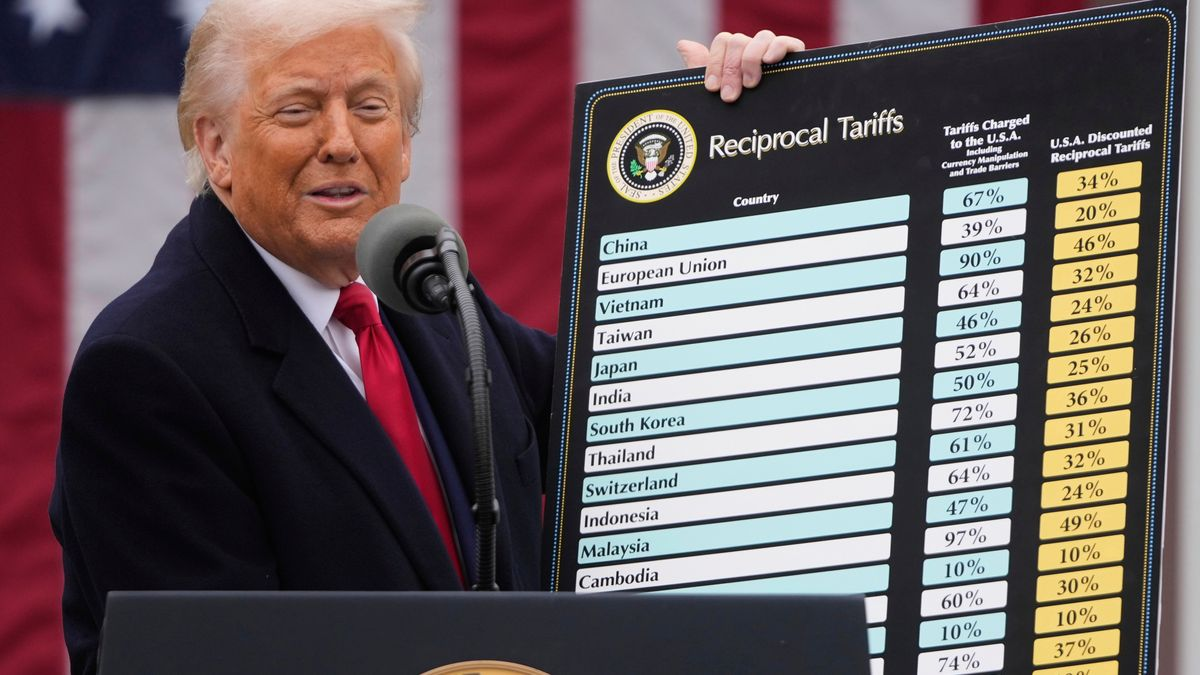
\includegraphics[keepaspectratio, height=\paperheight]{../img/trump_tariffs.jpg}};
  \end{tikzpicture}
\end{frame}
% ----------------------------------------------------
% IMAGE NEEDED: trump_tariffs.jpg -- fotografía de Trump firmando una orden ejecutiva sobre aranceles al acero o aluminio (2018 o 2025), o imagen de la rueda de prensa en la que anunció los aranceles globales de 2025; puede incluir la pancarta o el cartel con el porcentaje de aranceles por país
\note{Los aranceles de Trump al acero y aluminio (2018, 25\% y 10\% respectivamente) son el caso más reciente del ciclo de proteccionismo americano. En 2025, Trump volvió a imponer aranceles masivos, incluyendo tarifas del 10\% sobre casi todas las importaciones y aranceles recíprocos contra China (hasta el 145\%). El argumento oficial: proteger empleos industriales y reducir el déficit comercial. La respuesta económica: las industrias que usan acero (automóviles, construcción) vieron subir sus costes. Los socios comerciales tomaron represalias. El déficit comercial no mejoró. Pero políticamente, los aranceles conectan con votantes en el cinturón del óxido que sienten que el libre comercio los ha abandonado.}

% ====================================================
\section{Política doméstica}
% ====================================================

% ----------------------------------------------------
\begin{transitionframe}
La política doméstica del comercio
\end{transitionframe}
% ----------------------------------------------------
\note{}

% ----------------------------------------------------
\begin{frame}
\frametitle{Instituciones electorales y comercio}
\centering

\begin{itemize}
  \item Las instituciones electorales condicionan quién tiene influencia
  \vspace{4pt}
  \item \textbf{Circunscripciones locales} (EE.UU., UK):
  \begin{itemize}
    \item El representante defiende a las industrias de su distrito
    \item Aunque el coste sea nacional, el beneficio es local y visible
  \end{itemize}
  \vspace{4pt}
  \item<2-> \textbf{Listas de partido} (sistemas proporcionales):
  \begin{itemize}
    \item Menor presión sectorial directa
    \item Mayor coherencia de política comercial del partido
  \end{itemize}
  \vspace{4pt}
  \item<3-> Implicación: los sistemas mayoritarios tienden a \textbf{más proteccionismo sectorial}
\end{itemize}

\end{frame}
% ----------------------------------------------------
\note{El diseño institucional importa para la política comercial. En EE.UU., los congresistas representan distritos geográficos específicos. El senador de Pennsylvania tiene todos sus votantes en un estado con mucho acero y carbón. Tiene incentivos muy fuertes para apoyar la protección siderúrgica, aunque el coste para el resto del país sea mucho mayor. Este mecanismo se llama ``logrolling'': varios representantes se apoyan mutuamente en las protecciones sectoriales que interesan a sus distritos, aunque el resultado agregado sea más proteccionismo del que nadie querría en abstracto. En sistemas de listas de partido (como España o los países nórdicos), los diputados son menos vulnerables a este tipo de presión local. La teoría predice más libre comercio en sistemas proporcionales, y hay evidencia empírica que lo apoya.}

% ----------------------------------------------------
\begin{frame}
\frametitle{Partidos, clases y comercio}
\centering

\begin{columns}[T]
  \begin{column}{0.47\textwidth}
    \centering
    \textbf{\textcolor{accent}{Stolper-Samuelson}}
    \begin{itemize}
      \item Izquierda en países ricos: librecambistas (trabajo no es el factor escaso)
      \item Derecha en países ricos: proteccionistas (capital es factor escaso)
    \end{itemize}
  \end{column}
  \begin{column}{0.47\textwidth}
    \centering
    \textbf{\textcolor{accent2}{Realidad reciente}}
    \begin{itemize}
      \item Izquierda: cada vez más crítica con el libre comercio
      \item Derecha populista: \alert{proteccionista}
      \item Derecha tradicional: librecambista
    \end{itemize}
  \end{column}
\end{columns}

\vspace{10pt}
\onslide<2->{\small La política del comercio en el siglo XXI \textbf{no sigue las predicciones clásicas}}

\end{frame}
% ----------------------------------------------------
\note{La teoría de Stolper-Samuelson predice que en países ricos con abundancia de capital cualificado, la izquierda (que representa al trabajo) debería ser librecambista, porque el libre comercio beneficia a los trabajadores de países pobres (el factor abundante) y perjudica al capital de países pobres. La derecha, que representa al capital de países pobres, debería ser proteccionista. Pero en la práctica histórica, en EE.UU. en el siglo XX era al contrario: el Partido Republicano (de los intereses del capital) era librecambista, y los demócratas (sindicatos) eran más proteccionistas. Esto se explica porque el capital americano es abundante y se beneficia del libre comercio. Hoy el mapa ha vuelto a cambiar: el trumpismo rompe con el librecambismo republicano tradicional, y parte de la izquierda también es escéptica del libre comercio (por su impacto en los trabajadores manufactureros y las cadenas de valor).}

% ----------------------------------------------------
\begin{frame}
\frametitle{Backlash: el coste político de la globalización}
\centering

\begin{itemize}
  \item Desde 2008-2016: \textbf{reacción política contra la globalización}
  \vspace{8pt}
  \item Causas:
  \begin{itemize}
    \item ``China shock'': pérdida masiva de empleos manufactureros en EE.UU.
    \item Automatización + comercio = regiones industriales deprimidas
    \item Percepción de que las elites se beneficiaron, los trabajadores no
  \end{itemize}
  \vspace{8pt}
  \item<2-> Manifestaciones políticas:
  \begin{itemize}
    \item Trump (2016, 2024): aranceles, salida del TPP, renegociación del NAFTA
    \item Brexit (2016): ``recuperar el control'' de la política comercial
    \item Populismos europeos: crítica de los tratados de libre comercio (TTIP)
  \end{itemize}
\end{itemize}

\end{frame}
% ----------------------------------------------------
\note{El ``China shock'' es uno de los temas más estudiados en economía política reciente. Autor, Dorn y Hanson (2013, 2016) muestran que la entrada de China en la OMC (2001) tuvo efectos devastadores en regiones manufactureras específicas de EE.UU.: pérdida de entre 2 y 2,4 millones de empleos directos en manufactura. Las regiones más afectadas son exactamente las que bascularon hacia Trump en 2016. El ajuste del mercado laboral fue mucho más lento y doloroso de lo que predecían los modelos de comercio estándar. Esto ha generado un replanteamiento en la economía del comercio: las ganancias netas son reales, pero los costes locales y las disrupciones a corto plazo pueden ser políticamente insoportables. La pregunta política: ¿puede el libre comercio sobrevivir si los perdedores no son compensados?}

% ----------------------------------------------------
\begin{frame}
\frametitle{Compensar a los perdedores}
\centering

\begin{itemize}
  \item Si el libre comercio genera ganancias netas, se puede \textbf{compensar} a los perdedores
  \vspace{8pt}
  \item \textbf{Compensación teórica:} criterio de Kaldor-Hicks
  \begin{itemize}
    \item Los ganadores podrían compensar a los perdedores y aún ganar
    \item Pero la compensación raramente ocurre en la práctica
  \end{itemize}
  \vspace{8pt}
  \item<2-> \textbf{Instrumentos reales:}
  \begin{itemize}
    \item Estado de bienestar: seguro de desempleo, formación, sanidad
    \item \textit{Trade Adjustment Assistance} (TAA, EE.UU.): ayudas a trabajadores desplazados
    \item Fondos estructurales en la UE
  \end{itemize}
  \item<3-> \alert{Sin compensación efectiva, el libre comercio pierde apoyo político}
\end{itemize}

\end{frame}
% ----------------------------------------------------
\note{El criterio de Kaldor-Hicks establece que una política es eficiente si los ganadores podrían hipotéticamente compensar a los perdedores y aún así quedar mejor. El libre comercio generalmente cumple este criterio: las ganancias de los consumidores y los sectores exportadores superan las pérdidas de los sectores que compiten con importaciones. Pero ``hipotéticamente'' es la palabra clave: la compensación no ocurre automáticamente. El Trade Adjustment Assistance (TAA) en EE.UU. existe desde 1962, pero su financiación siempre ha sido insuficiente y sus beneficios limitados. Los países europeos con estados de bienestar robustos han tenido menos backlash político contra la globalización, porque los perdedores tienen redes de seguridad (Dinamarca, los países nórdicos). La paradoja: EE.UU., que más promovió el libre comercio global, tiene un estado de bienestar demasiado débil para compensar a sus propios perdedores.}

% ====================================================
\section{Cooperación internacional}
% ====================================================

% ----------------------------------------------------
\begin{transitionframe}
Cooperación internacional y la OMC
\end{transitionframe}
% ----------------------------------------------------
\note{}

% ----------------------------------------------------
\begin{frame}
\frametitle{El dilema del prisionero en el comercio}
\centering
\vspace{0.5em}

\begin{tikzpicture}[>=stealth]
  % Matrix (shifted right to avoid left margin clipping)
  \node at (4.5, 3.2) {\textbf{País B}};
  \node at (2.3, 3.2) [font=\small, text=accent] {Libre comercio};
  \node at (6.4, 3.2) [font=\small, text=accent2] {Proteccionismo};

  \node at (0.8, 1.4) {\textbf{País A}};
  \node at (0.5, 2.0) [font=\small, text=accent] {Libre};
  \node at (0.5, 0.7) [font=\small, text=accent2] {Protec.};

  \draw (1,0) grid[step=2] (7.8, 2.8);

  \node at (2.7, 2.1) [font=\small] {+3, +3};
  \node at (6.1, 2.1) [font=\small, text=accent2] {-1, +4};
  \node at (2.7, 0.7) [font=\small, text=accent2] {+4, -1};
  \node at (6.1, 0.7) [font=\small, text=accent2] {0, 0};

  \node at (2.7, 1.5) [font=\scriptsize, text=asher] {óptimo};
  \node at (6.1, 0.3) [font=\scriptsize, text=accent2] {equilibrio};
\end{tikzpicture}

\vspace{6pt}
{\scriptsize (cada celda: beneficio País A, beneficio País B)}

\end{frame}
% ----------------------------------------------------
\note{La lógica del dilema del prisionero aplicada al comercio. Si ambos países eligen libre comercio, ambos ganan (3,3). Pero cada uno tiene incentivo a ``hacer trampa'': si el otro abre su mercado y yo lo cierro, me llevo 4 a su -1. El equilibrio sin cooperación es (0,0): ambos proteccionistas. Esta es exactamente la lógica de las guerras comerciales: si yo pongo aranceles y tú no, te saco ventaja. Si tú pones aranceles y yo no, te sale más barato que a mí. El resultado: nos enzarzamos en guerras de aranceles que nos dejan a ambos peor. La solución: mecanismos de cooperación que hagan que la defección sea costosa. Eso es exactamente lo que hace el GATT/OMC.}

% ----------------------------------------------------
\begin{frame}
\frametitle{Del GATT a la OMC}
\centering
\vspace{0.5em}

\begin{tikzpicture}[>=stealth, thick]
  % Timeline
  \draw[thick] (0,0) -- (10,0);

  % Ticks and labels
  \foreach \x/\y/\lab in {
    0/above/1947,
    3.5/above/1979,
    6/above/1995,
    9/above/2001
  } {
    \draw (\x, -0.15) -- (\x, 0.15);
    \node[\y, font=\footnotesize] at (\x, 0.2) {\lab};
  }

  % Events below the line
  \node[below, font=\scriptsize, align=center] at (0, -0.2) {Firma del\\GATT};
  \node[below, font=\scriptsize, align=center] at (3.5, -0.2) {Ronda de\\Tokio};
  \node[below, font=\scriptsize, align=center] at (6, -0.2) {Creación\\de la OMC};
  \node[below, font=\scriptsize, align=center] at (9, -0.2) {China\\ingresa};

  % Band showing tariff reductions
  \fill[accent!30, opacity=0.5] (0, 0.5) rectangle (10, 1.0);
  \node[font=\scriptsize, align=center] at (5, 0.75) {De $\sim$40\% (1947) a $\sim$5\% (2000)};
\end{tikzpicture}

\vspace{10pt}
\small El GATT (1947) fue el primer marco multilateral para la liberalización comercial

\end{frame}
% ----------------------------------------------------
\note{El GATT (Acuerdo General sobre Aranceles Aduaneros y Comercio) fue firmado en 1947 por 23 países. Nació del desastre del período de entreguerras: la Gran Depresión llevó a los países a una espiral de aranceles (la Ley Smoot-Hawley de 1930 subió los aranceles americanos al 45\%, los socios tomaron represalias, el comercio mundial se desplomó un 65\% entre 1929 y 1934, lo que agravó la depresión). El GATT era una institución ligera: no tenía personalidad jurídica propia, sino que era un conjunto de acuerdos. Se articulaba en ``rondas'' de negociación. Las primeras rondas se centraron en aranceles industriales (fáciles de cuantificar y negociar). La Ronda Kennedy (1964-67) y la Ronda Tokio (1973-79) ampliaron las reducciones. La Ronda Uruguay (1986-94) fue la más ambiciosa: creó la OMC, incorporó servicios (GATS), propiedad intelectual (TRIPS) y agricultura.}

% ----------------------------------------------------
\begin{frame}
\frametitle{La OMC: principios y mecanismos}
\centering
\small
\begin{itemize}
  \item \textbf{Nación más favorecida (NMF):}
  \begin{itemize}
    \item Si das una ventaja a un país, debes dársela a todos los miembros
    \item Prohíbe la discriminación bilateral
  \end{itemize}
  \item<2-> \textbf{Reciprocidad:}
  \begin{itemize}
    \item Las concesiones se negocian de forma equilibrada
    \item Soluciona el dilema del prisionero: ambos abren al mismo tiempo
  \end{itemize}
  \item<3-> \textbf{Resolución de disputas:}
  \begin{itemize}
    \item Órgano de Solución de Diferencias (OSD)
    \item Los países pueden impugnar políticas de otros miembros
    \item Autoriza sanciones si se incumple el laudo
  \end{itemize}
  \item<4-> 164 miembros (2024) --- \alert{casi universal}
\end{itemize}

\end{frame}
% ----------------------------------------------------
\note{Los tres principios fundacionales de la OMC. (1) Nación más favorecida (NMF o MFN en inglés): es la cláusula de no discriminación. Si EE.UU. reduce el arancel sobre los coches alemanes al 5\%, debe aplicar ese mismo 5\% a todos los miembros de la OMC. Esto generaliza automáticamente las concesiones bilaterales y es la razón de que el GATT haya podido reducir aranceles globalmente con negociaciones entre unos pocos países grandes. (2) Reciprocidad: resuelve el dilema del prisionero. No se trata de que un país abra su mercado unilateralmente; los países negocian aperturas simultáneas. Esto hace políticamente posible conceder acceso a mercados extranjeros: el gobierno puede decir a sus productores ``abrimos, pero a cambio de acceso para nuestros exportadores.'' (3) Resolución de disputas: el OSD de la OMC es uno de los tribunales internacionales más activos y eficaces. Ha habido más de 600 casos desde 1995. Los laudos se cumplen en la mayoría de los casos, aunque EE.UU. bajo Trump bloqueó el nombramiento de nuevos árbitros del Órgano de Apelación.}

% ----------------------------------------------------
\begin{frame}
\frametitle{Los límites de la cooperación comercial}
\centering

\begin{itemize}
  \item La OMC ha logrado \textbf{reducir aranceles} enormemente
  \vspace{8pt}
  \item Pero enfrenta retos crecientes:
  \begin{itemize}
    \item Barreras no arancelarias: difíciles de negociar
    \item Acuerdos regionales (TLC): proliferan, crean ``espagueti de normas''
    \item Ronda de Doha (2001--): \alert{bloqueada} por agricultura y servicios
    \item EE.UU. bloquea el Órgano de Apelación desde 2017
  \end{itemize}
  \vspace{8pt}
  \item<2-> Tensión entre \textbf{libre comercio} y \textbf{política industrial nacional}
  \begin{itemize}
    \item Subsidios estatales chinos (acero, energía solar)
    \item Inflation Reduction Act (EE.UU., 2022): subsidios a coches eléctricos
  \end{itemize}
\end{itemize}

\end{frame}
% ----------------------------------------------------
\note{La OMC tiene un éxito innegable en la reducción de aranceles: de una media del 40\% en 1947 a menos del 5\% en los países desarrollados en 2000. Pero desde la Ronda Uruguay no ha habido grandes acuerdos multilaterales. La Ronda de Doha (iniciada en 2001) lleva más de 20 años sin cerrarse, bloqueada principalmente por el desacuerdo entre los países desarrollados (que quieren abrir mercados de servicios y manufactura) y los países en desarrollo (que exigen reducción de subsidios agrícolas y acceso a medicamentos genéricos). El reto de los subsidios estatales es nuevo: la política industrial china y ahora la americana (IRA de 2022) son difícilmente compatibles con las normas de la OMC. Los acuerdos regionales (TLC bilaterales y plurilaterales) proliferan como alternativa, pero crean un sistema fragmentado con diferentes normas para diferentes socios.}

% ====================================================
\section{El trilema de la globalización}
% ====================================================

% ----------------------------------------------------
\begin{transitionframe}
El trilema de Rodrik
\end{transitionframe}
% ----------------------------------------------------
\note{}

% ----------------------------------------------------
\begin{frame}
\frametitle{El trilema de la globalización (Rodrik)}
\centering
\vspace{0.2em}

\begin{tikzpicture}[>=stealth, scale=0.9]
  % Triangle vertices
  \coordinate (A) at (0, 3.5);
  \coordinate (B) at (-3.5, 0);
  \coordinate (C) at (3.5, 0);

  % Triangle sides
  \draw[thick] (A) -- (B) -- (C) -- cycle;

  % Vertex labels
  \node[above, font=\small\bfseries] at (A) {Hiperglobalización};
  \node[left, font=\small\bfseries, align=right] at (B) {Soberanía\\nacional};
  \node[right, font=\small\bfseries, align=left] at (C) {Democracia};

  % Pair examples on each side
  \node[left, font=\scriptsize, text=accent, align=center] at (-1.75, 1.75)
    {``Camisa de fuerza\\dorada''};
  \node[below, font=\scriptsize, text=asher, align=center] at (0, -0.15)
    {Bretton Woods\\(1945--1973)};
  \node[right, font=\scriptsize, text=accent2, align=center] at (1.75, 1.75)
    {Gobernanza\\global federal};
\end{tikzpicture}

\vspace{4pt}
{\small Rodrik (2011): \alert{solo puedes tener dos de los tres}}

\end{frame}
% ----------------------------------------------------
\note{Dani Rodrik formuló este trilema en \textit{The Globalization Paradox} (2011). La idea es análoga al trilema monetario: no puedes tener las tres cosas a la vez. Si quieres hiperglobalización (integración económica profunda) y soberanía nacional, tienes que limitar la democracia: aceptar las reglas del mercado global sin importar lo que quieran los votantes (la ``camisa de fuerza dorada'' de Thomas Friedman). Si quieres hiperglobalización y democracia, necesitas gobernanza global democrática (un gobierno federal mundial), lo cual no existe. Si quieres soberanía nacional y democracia, tienes que aceptar límites a la integración económica: es el compromiso de Bretton Woods, comercio abierto pero con controles de capital y margen para políticas nacionales.}

% ----------------------------------------------------
\begin{frame}
\frametitle{El trilema y el momento actual}
\centering

\begin{itemize}
  \item Desde los 90: la tendencia fue \textbf{hiperglobalización + soberanía}
  \begin{itemize}
    \item Integración profunda con poca compensación interna
    \item La ``camisa de fuerza dorada'': adaptarse al mercado global o quedarse atrás
  \end{itemize}
  \vspace{8pt}
  \item<2-> Resultado: la \textbf{democracia} reaccionó
  \begin{itemize}
    \item Trump, Brexit, populismos: los votantes rechazan la globalización sin compensación
    \item Las democracias exigen soberanía \textbf{y} rendición de cuentas
  \end{itemize}
  \vspace{8pt}
  \item<3-> La propuesta de Rodrik: una globalización \textbf{más modesta}
  \begin{itemize}
    \item Bretton Woods permitía comercio abierto con margen para políticas nacionales
    \item Las democracias deben poder proteger su contrato social
    \item No es ``anti-globalización'': es globalización \alert{compatible con la democracia}
  \end{itemize}
\end{itemize}

\end{frame}
% ----------------------------------------------------
\note{La evolución de los últimos 30 años se puede leer a través del trilema de Rodrik. En los años 90 y 2000, el consenso de Washington promovió la hiperglobalización: libre comercio profundo, libre movimiento de capitales, y adaptación de las políticas nacionales a las exigencias del mercado global. Esto sacrificó de facto la capacidad de las democracias nacionales para elegir sus propias políticas económicas. La reacción populista (Trump, Brexit, pero también Syriza en Grecia o los chalecos amarillos en Francia) es la democracia reclamando su espacio: los votantes dicen ``no queremos más integración si eso significa que no podemos elegir nuestras propias políticas.'' Rodrik no propone cerrar fronteras, sino volver al espíritu de Bretton Woods: comercio abierto, pero con espacio para que cada país mantenga sus instituciones. La globalización no debería requerir la armonización total de las políticas domésticas.}

% ----------------------------------------------------
\begin{frame}
\frametitle{Resumen}
\centering
\vspace{1em}

\begin{itemize}
  \setlength{\itemsep}{8pt}
  \item El libre comercio genera \textbf{ganancias netas}, pero también ganadores y perdedores
  \item La \textbf{ventaja comparativa} explica la especialización; H-O explica los patrones
  \item Los perdedores del comercio están \textbf{mejor organizados} que los ganadores
  \item El proteccionismo responde a lógicas políticas, no solo económicas
  \item La \textbf{OMC} resuelve el dilema del prisionero mediante reciprocidad y NMF
  \item El \textbf{trilema de Rodrik}: no se puede tener hiperglobalización, soberanía y democracia a la vez
\end{itemize}

\end{frame}
% ----------------------------------------------------
\note{Resumen de los conceptos clave de la sesión. La pregunta central (¿por qué los gobiernos restringen el comercio si genera ganancias netas?) tiene dos respuestas: (1) los perdedores están mejor organizados que los ganadores (acción colectiva); (2) las ganancias son difusas y las pérdidas concentradas. La OMC ayuda a superar el dilema del prisionero mediante la reciprocidad y la no discriminación, pero enfrenta límites crecientes. El trilema de Rodrik ofrece un marco para entender el debate actual: la hiperglobalización de los años 90 sacrificó la capacidad de las democracias nacionales para elegir sus propias políticas, y la reacción populista es la democracia reclamando su espacio.}

% ----------------------------------------------------
\begin{frame}
\centering
\vspace{2em}
{\large ¿Es posible mantener el libre comercio\\[10pt]
sin un estado de bienestar que compense\\[6pt]
a los perdedores de la globalización?}
\end{frame}
% ----------------------------------------------------
\note{Pregunta de cierre. La evidencia comparada sugiere que los países nórdicos han podido mantener apertura comercial porque tienen redes de seguridad robustas. EE.UU. ha promovido el libre comercio globalmente pero tiene un estado de bienestar débil --- y el resultado es el backlash político que vemos. El dilema: para aprobar políticamente el libre comercio necesitas compensar a los perdedores, pero la redistribución también requiere coaliciones políticas difíciles de construir. Adelanto para la próxima sesión: el trilema de Rodrik tiene un primo hermano en las finanzas internacionales --- el trilema monetario. Veremos que tampoco se puede tener tipo de cambio fijo, libre movimiento de capitales y política monetaria autónoma al mismo tiempo. La misma lógica de restricciones imposibles, aplicada al dinero.}
